
%(BEGIN_QUESTION)
% Copyright 2010, Tony R. Kuphaldt, released under the Creative Commons Attribution License (v 1.0)
% This means you may do almost anything with this work of mine, so long as you give me proper credit

Calculate the amount of voltage ``seen'' by the voltmeter given the following measurement and reference junction temperatures:

$$\includegraphics[width=15.5cm]{i02945x01.eps}$$

\begin{itemize}
\item{} $T_{1}$ = 233 $^{o}$C ; $T_{2}$ = 31 $^{o}$C ; $T_3$ = 25 $^{o}$C ; $V_{meter}$ = \underbar{\hskip 50pt} mV
\vskip 10pt
\item{} $T_{1}$ = 348 $^{o}$C ; $T_{2}$ = 40 $^{o}$C ; $T_3$ = 16 $^{o}$C ; $V_{meter}$ = \underbar{\hskip 50pt} mV
\vskip 10pt
\item{} $T_{1}$ = $-161$ $^{o}$C ; $T_{2}$ = $-4$ $^{o}$C ; $T_3$ = 23 $^{o}$C ; $V_{meter}$ = \underbar{\hskip 50pt} mV
\vskip 10pt
\item{} $T_{1}$ = 836 $^{o}$C ; $T_{2}$ = 34 $^{o}$C ; $T_3$ = 19 $^{o}$C ; $V_{meter}$ = \underbar{\hskip 50pt} mV
\end{itemize}

\underbar{file i02945}
%(END_QUESTION)





%(BEGIN_ANSWER)

All answers based on ITS-90 thermocouple table values:

\begin{itemize}
\item{} $T_{1}$ = 233 $^{o}$C ; $T_{2}$ = 31 $^{o}$C ; $T_3$ = 25 $^{o}$C ; $V_{meter}$ = {\bf 14.395} mV
\vskip 10pt
\item{} $T_{1}$ = 348 $^{o}$C ; $T_{2}$ = 40 $^{o}$C ; $T_3$ = 16 $^{o}$C ; $V_{meter}$ = {\bf 23.856} mV
\vskip 10pt
\item{} $T_{1}$ = $-161$ $^{o}$C ; $T_{2}$ = $-4$ $^{o}$C ; $T_3$ = 23 $^{o}$C ; $V_{meter}$ = {\bf $-$9.039} mV
\vskip 10pt
\item{} $T_{1}$ = 836 $^{o}$C ; $T_{2}$ = 34 $^{o}$C ; $T_3$ = 19 $^{o}$C ; $V_{meter}$ = {\bf 62.701} mV
\end{itemize}

Note: all temperatures at $T_2$ are irrelevant because this is a junction between similar metals (type E wires connecting to corresponding type EX extension wires).  The reference (cold) junction is where the type EX wires connect to copper, at temperature $T_3$.

%(END_ANSWER)





%(BEGIN_NOTES)


%INDEX% Measurement, temperature: thermocouple 

%(END_NOTES)

